\section{Extending \t{sg-web}}

  When running \program{sg-web} it can be made aware of additional Scheme modules and
  resources by modifying three environment variables:
  \t{SG\_WEB\_ROOT}, \t{GUILE\_LOAD\_PATH}, and \t{GUILE\_LOAD\_COMPILED\_PATH}.

  To ensure normal operation, \program{sg-web} prefers its own resources
  before considering extensions.  Therefore files shipped with SPARQLing-genomics
  cannot be overridden.

\subsection{Scheme code}

  There are pre-defined areas in which \program{sg-web} can be extended.  Each
  area dictates a module prefix.  For example, a \emph{form} module is searched
  for in the ``\t{www forms}'' prefix, which means that the module's file must
  be located in the subdirectory \t{www/forms}, relative to the path that
  \t{GUILE\_LOAD\_PATH} and \t{GUILE\_LOAD\_COMPILED\_PATH} point to.

\subsection{Static resources}

  When the Scheme code refers to static resources that are not part of
  SPARQLing-genomics (like an image file or additional JavaScript files),
  they must be added to the \t{SG\_WEB\_ROOT}.  Additionally, the path added to
  \t{SG\_WEB\_ROOT} must point to a path that contains the subdirectory
  \t{static}.

  The following example illustrates how this works.  Consider the following
  SXML code to display an image.
\begin{siderules}
\begin{verbatim}
(img (@ (src "/static/example-image.jpg") (alt "Example")))
\end{verbatim}
\end{siderules}

  It refers to a file called \t{static/example-image.jpg}.  Let's further
  assume that this file is located on our filesystem at
  \t{/home/user/form-module/static/example-image.jpg}.

  For \program{sg-web} to find this resource, we need to set \t{SG\_WEB\_ROOT}
  as the following:
\begin{siderules}
\begin{verbatim}
export SG_WEB_ROOT=/home/user/form-module
\end{verbatim}
\end{siderules}

\section{Forms}
\label{sec:forms}

  Forms provide a mechanism to gather input from users.  Form modules must be
  placed under the \t{www forms} prefix.  Creating a web form that leverages
  SPARQLing-genomics involves creating a Scheme module that implements three
  procedures:
  \begin{itemize}
  \item \t{page}: This procedure should return an SXML tree that represents
    the HTML to display the form.
  \item \t{submit}: This procedure implements the action to take when a user
    submits the form.
  \item \t{api}: This optional procedure can be used to build autocompletion,
    or other pre-submit interaction between the form and SPARQLing-genomics.
  \end{itemize}

\subsection{Example of a form module}

  Creating a Scheme module to render a form to users comprises of four
  parts.  In the remainder of this section we will address each part.

\subsubsection{The Scheme module}
\label{sec:scheme-module}

  The first part involves defining a Scheme modules with three procedures.
  Because \program{sg-web} is written in GNU Guile \citep{guile},
  we use \t{define-module} to define the module for the form.

\begin{siderules}
\begin{verbatim}
(define-module (www forms example)
  #:use-module (www pages) ; Provides the ‘page-empty-template’ procedure.
  #:use-module (www util)  ; Provides the ‘string-is-longer-than’ procedure.
  #:export (page submit api))
\end{verbatim}
\end{siderules}

  Because the name of the module is \t{(www forms example)}, the location
  where \program{sg-web} searches for your module is `\t{www/forms/example.scm}'
  relative to a path on \t{GUILE\_LOAD\_PATH}.  The ``\t{www forms}'' module
  prefix is hard-coded by \program{sg-web}, while \t{example} can be chosen by
  us.

  There are three symbols we export from our module: \t{page}, \t{submit}, and
  \t{api}.  The \program{sg-web} expects these exact symbol names to be
  exported.

\subsubsection{Implementing the \t{page} procedure}

  The second part involves implementing the \t{page} procedure. The \t{page}
  procedure takes the request path and request parameters as arguments
  (ignoring optional arguments), returning an SXML tree.  The request path
  can be used to tell where to submit the form to.

\begin{siderules}
\begin{verbatim}
(define* (page request-path arguments #:optional (error-message #f))
  (page-empty-template "Example" request-path
   `((h2 "Example form")
     ,(if error-message
         `(div (@ (class "form-error-message")) ,error-message)
         '())

     (form (@ (method "POST")
              (action ,request-path))
       (h3 "Name")
       (input (@ (type  "text")
                 (id    "name")
                 (name  "name")))
       (input (@ (type  "submit")
                 (class "form-submit-button")
                 (value "Submit form")))))))
\end{verbatim}
\end{siderules}

  The \t{(www pages)} module provides a template that includes the familiar
  theme of the \program{sg-web} pages.  Our SXML tree will render to the
  following HTML:

\begin{siderules}
\begin{verbatim}
<h2>Example form</h2>
<form method="POST" action="/forms/example">
  <h3>Name</h3>
  <input type="text" id="name" name="name" />
  <input type="submit" class="form-submit-button" value="Submit form" />
</form>
\end{verbatim}
\end{siderules}

  Note that this HTML snippet is wrapped inside the template constructed by
  \t{page-empty-template}, so when viewing the form in a web browser, we
  will see something similar to figure \ref{fig:web-form-example}.

  \begin{figure}[H]
    \begin{center}
      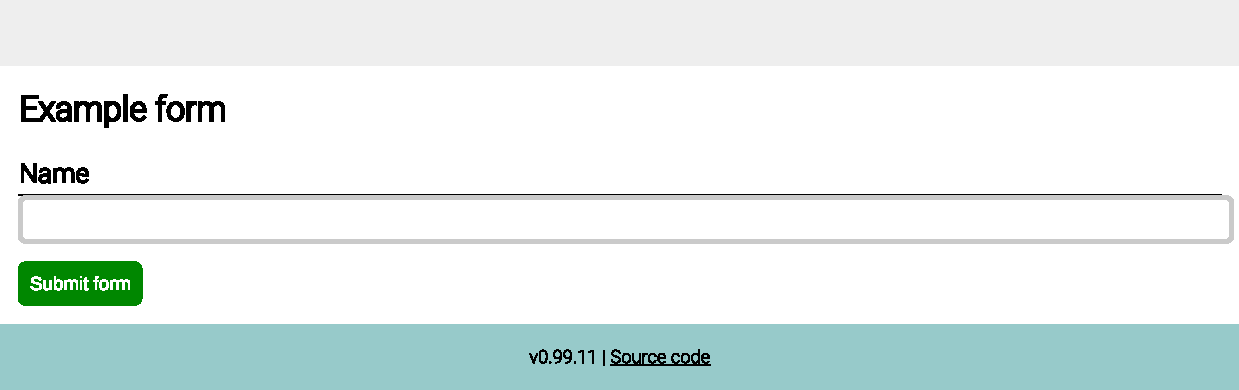
\includegraphics[width=1.0\textwidth]{figures/sg-web-form-example.pdf}
    \end{center}
    \caption{The rendering of the \t{page} procedure of our example form.}
    \label{fig:web-form-example}
  \end{figure}

\subsubsection{Implementing the \t{submit} procedure}

  The third step is to catch a form submission, which is the purpose of the
  \t{submit} procedure.  This procedure is expected to take two arguments,
  and return an SXML tree.

\begin{siderules}
\begin{verbatim}
(define (submit request-path data)
  (let* ((name (assoc-ref data 'name))
         (state (cond
                 [(or (not name)
                      (not (string-is-longer-than name 0)))
                  '(#f "Missing name.")]
                 [(string-is-longer-than name 64)
                  '(#f "Name may not be longer than 64 characters.")]
                 [else
                  '(#t)])))
    (if (car state)
        (page-empty-template "Thank you" request-path
         `((h2 "Thank you, " ,name "!")))
        (page request-path #f (cadr state)))))
\end{verbatim}
\end{siderules}

  After submitting the form, it may render in the web browser as displayed
  in figure \ref{fig:web-form-submit}.

  \begin{figure}[H]
    \begin{center}
      
\includegraphics[width=1.0\textwidth]{figures/sg-web-form-example-submit.pdf}
    \end{center}
    \caption{The rendering of the \t{submit} procedure of our example form.}
    \label{fig:web-form-submit}
  \end{figure}


\subsubsection{Implementing the \t{api} procedure}

  The final step involves implementing the optional \t{api} procedure
  that takes seven arguments:
  \begin{itemize}
  \item \t{request-path}:   The relative path of the form;
  \item \t{arguments}:      An alist of parameters passed by the URI.
  \item \t{input-port}:     The port to read data from;
  \item \t{output-port}:    The port to write data to;
  \item \t{accept-type}:    The value of the requests's \t{Accept} header;
  \item \t{content-type}:   The value of the requests's \t{Content-Type} header;
  \item \t{content-length}: The number of bytes that can be read from
    \t{input-port}.
  \end{itemize}

  This procedure is primarily designed to provide autocompletion options
  for form fields.

\begin{siderules}
\begin{verbatim}
(define (api request-path arguments input-port output-port
             accept-type content-type content-length)
  ...)
\end{verbatim}
\end{siderules}

\pagebreak{}
\section{Reports}
\label{sec:reports}

  Reports are displayed in the ``report'' section of a project.  To implement
  a report module, the following variables and procedures need to be implemented:
  \begin{itemize}
  \item \t{title}: The title for the subheading in the ``report'' page.
  \item \t{project}: The hash of the project to display the report module.
  \item \t{report-overview}: A procedure that returns an SXML tree that
    provides the content under the subheading of the report module.
  \end{itemize}

\subsection{Example of a report module}

  Report modules must be placed under the \t{www reports} module prefix.

\subsubsection{The Scheme module}
\label{sec:scheme-module}

  The first part involves defining a Scheme modules with one procedure and
  two variables.

\begin{siderules}
\begin{verbatim}
(define-module (www reports example)
  #:export (title project report-overview))
\end{verbatim}
\end{siderules}

\subsubsection{Implementing \t{title} and \t{project}}

  Setting \t{title} and \t{project} involves defining two variables.

\begin{siderules}
\begin{verbatim}
(define title   "Example report")
(define project "e434cfe3752025c6fdbedbccc3f25265198da4358b0e23c77897bf7f5844ba5c")
\end{verbatim}
\end{siderules}

  Upon entering the \emph{Report} page, \t{sg-web} displays only the report
  modules that are configured for the current project.  Therefore it is
  important to ensure the value set in \t{project} matches the
  \emph{project hash} of the project intended to extend.

\subsubsection{Implementing the \t{report-overview} procedure}

  The \t{report-overview} procedure takes no argments and is expected to
  return an SXML tree that renders HTML.  The following implementation of
  the \t{report-overview} procedure renders a table.

\begin{siderules}
\begin{verbatim}
(define (report-overview)
  `(table (@ (class "item-table"))
     (tr (th "Identifier")
         (th "Description"))
     (tr (td "foo")
         (td "bar"))))
\end{verbatim}
\end{siderules}

